%-------
% Notes
%   ~ADD       : Add the following.
%   ~REFERENCE : Reference the following paper/authors.
%   ~FIND      : Find a paper regarding the following.
%   ~CHECK     : Check that the following is met.
%   ~READ      : Read through the following paper/authors.
%   ~MENTION   : Mention the following.
%   ~AMMEND    : Make a change to the following.
%   ~IDEA      : Suggestion for later in the project.

\documentclass{UoYCSproject}
\usepackage{geometry}

% -----------
% Tikz Setup 
\usepackage{tikz}
\usetikzlibrary{ matrix,      % For easy node positioning
                 fit,         % For easily fitting nodes inside another one
                 arrows,
                 positioning, % For easy node-relative placements
               }
\tikzstyle{edge} = [->, bend left]
\tikzstyle{edge'} = [->, bend right]
\tikzstyle{vertex} = [circle, minimum width=0.5cm, text centered, draw=black]
\tikzstyle{graph_small} = [rectangle, draw=black, inner sep=0.5cm]
\tikzstyle{graph} = [rectangle, draw=black, inner sep=1cm]
\tikzstyle{rule} = [rectangle, inner sep=1cm]
\tikzstyle{derivation} = [-implies, double, thick]

% ---------------
% Listings Setup
\usepackage{listings}
\renewcommand{\lstlistingname}{C Code}

\author{Huw Taylor}
\title{Tracing GP2 Execution} %TODO ~AMMEND: is 'Execution' needed? Maybe just Tracing GP2?
\date{\today}
\supervisor{Dr. Detlef Plump}
\MEng
%TODO ~CHECK: The word/page counts are up to date.
\wordcount{-1}
\pagecount{-1}
% ~16000 words (55 pages) total
\abstract{
% ~66 words

}
\acknowledgements{
I would like to thank Christopher Bak for his support throughout the project. His advice on the workings of the GP2 compiler has been invaluable.
% Detlef?
}

\begin{document}

\maketitle
\tableofcontents
% \listoffigures

\chapter{Introduction}
% ~1333 words
\section{Motivation}
GP is a graph programming language. It was developed to provide a language that is expressive enough to solve complex graph problems, while also having a simple enough syntax to allow for formal reasoning. Graphs and graph transformations have previously implemented in low-level languages, like C. This meant that it was more difficult to understand, verify, and implement\cite{gp_lang}. GP at its core has four commands that nevertheless allows every computable function on graphs to be implemented \cite{gp1}. These commands are a single application of a rule, sequential composition, loops, and branching. Loops are implemented in a run-for-as-long-as-possible style.
%TODO ~ADD: more stuff about GP (page 18 on https://www.cs.york.ac.uk/ftpdir/reports/2007/YCST/15/YCST-2007-15.pdf (gp_lang) and page 1 on https://www.cs.york.ac.uk/plasma/publications/pdf/Plump.CAI.09.pdf (gp1))

GP2, the second iteration of GP, builds upon the first. It adds the marking of nodes with a colour, or a special 'any' colour; additional conditions that can be checked against in a rule's schema, including the indegree and outdegree of an edge, and whether there exists an edge between two nodes; and an additional branching mechanism: a try-then-else. In try-then-else and if-then-else branching, the condition is a set of rules schemata, and often alters the graph. If-then-else branching uses the graph before the 'if' condition is evaluated, and any changes are made, in the 'then' branch. In contrast, the try-then-else uses the \emph{result} of the 'try' condition in the 'then' branch. In both, the 'else' branch uses the graph before the condition is checked against \cite{gp2_design}.
%TODO ~ADD: what GP2 adds (page 1 on https://www.cs.york.ac.uk/plasma/publications/pdf/Plump.WRS.11.pdf (gp2_design))

The University of York has produced a compiler for GP2. %TODO ~MENTION: a bit about the compiler. Doesn't have non-determinism properly, or rather doesn't allow for full exploration of the solution space.

The University of York has produced a graphical editor for creating graphs and graph programs. The editor depends on the compiler to execute the program on the host graph, thereby producing the resultant graph. It displays the graphs %TODO ~ADD: say more about the editor. The horrible horrible editor.

The aim of this project is to show the execution of the program. As it is, the entire program is run, and the resulting graph is saved. This project aims to show the intermediate steps of the program. This will allow the correctness of the program to be ensured, and also so that people using these tools, who may not have a complete understanding of how graph programs work, can see the process with a finer granularity.

%TODO ~ADD: The benefits of being able to step through programs. 

\section{Ethics}
The project discussed has very few ethical considerations. It is not related to defence and there are no safety or security concerns. No humans or animals are involved in its development.

\chapter{Literature Review}
% ~4000 words
%TODO ~CHECK: Shows that you know what is happening in your field 
%TODO ~CHECK: Justifies why your work is interesting or important 
%TODO ~CHECK: establishes the theoretical framework/context for your work 
%TODO ~CHECK: defends your choice of methodology 
%TODO ~CHECK: avoids repeating previous researchers’ mistakes
\section{Graph Programming}
\subsection{Graph Transformations}
A graph is a visual way of representing data and relationships. The formal definition is a set of vertices (nodes) \emph{V}, a set of edges \emph{E}, and a set of labels \emph{L}. Additionally \emph{source} and \emph{target} functions associate edges with nodes, and a \emph{label} function, which assigns labels to edges and nodes.
Graph theory is said to go back as far as the 1730s, with The K{\"o}nigsberg Bridge problem being regarded as the topic for the first paper on graph theory ever written \cite{grathe_origin}. %TODO ~ADD: references to double-pushout and single-pushout methods, as well as contributions to graph theory in general
The mathematical theory of Graph Transformation allows the transformation of graphs by way of rules. Rules are applied to graphs. They include a LHS (Left-Hand Side) graph, and RHS (Right-Hand Side) graph and an interface graph, which connects nodes in the LHS to nodes in the RHS. There is a convention that if the interface graph is ommited then it is inferred that it comprises the common labelled nodes in both the LHS and RHS.

Figure \ref{fig:simple_rule} on page \pageref{fig:simple_rule} shows a simple rule that, given a non-empty host graph, creates a transitive graph, where every node accessible by another has a direct edge going to it. Figure \ref{fig:simple_rule_sans_k} on page \pageref{fig:simple_rule_sans_k} shows the same rule without its interface graph.

%TODO ~ADD: "construction of rule application" how a rule works. Find the match, apply the rule. Morphisms and pushouts, which will be explained by this point.

\begin{figure}
\label{fig:simple_rule}
\centering
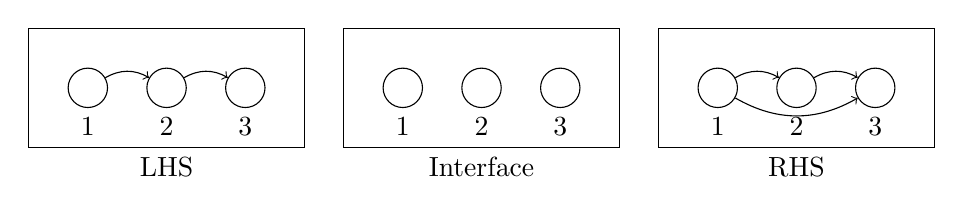
\begin{tikzpicture}[scale=2]
  \node (n1) [vertex, label=below:{1}] at (0, 0) {};
  \node (n2) [vertex, label=below:{2}] at (0.5, 0) {};
  \node (n3) [vertex, label=below:{3}] at (1, 0) {};
  \path [edge] (n1) edge node {} (n2);
  \path [edge] (n2) edge node {} (n3);
  \node (l) [graph_small, fit={(n1) (n2) (n3)}, label=below:{LHS}] {};
  
  \node (n4) [vertex, label=below:{1}] at (2, 0) {};
  \node (n5) [vertex, label=below:{2}] at (2.5, 0) {};
  \node (n6) [vertex, label=below:{3}] at (3, 0) {};
  \node (k) [graph_small, fit={(n4) (n5) (n6)}, label=below:{Interface}] {};
  
  \node (n7) [vertex, label=below:{1}] at (4, 0) {};
  \node (n8) [vertex, label=below:{2}] at (4.5, 0) {};
  \node (n9) [vertex, label=below:{3}] at (5, 0) {};
  \path [edge] (n7) edge node {} (n8);
  \path [edge] (n8) edge node {} (n9);
  \path [edge'] (n7) edge node {} (n9);
  \node (r) [graph_small, fit={(n7) (n8) (n9)}, label=below:{RHS}] {};
\end{tikzpicture}
\caption{Rule Example}
\end{figure}

\begin{figure}
\label{fig:simple_rule_sans_k}
\centering
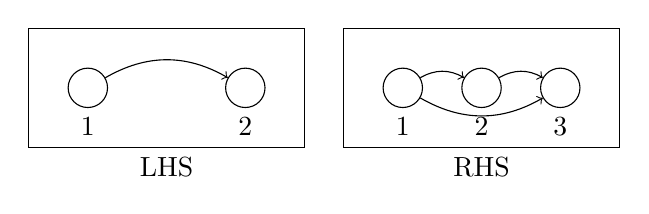
\begin{tikzpicture}[scale=2]
  \node (n1) [vertex, label=below:{1}] at (0, 0) {};
  \node (n2) [vertex, label=below:{2}] at (1, 0) {};
  \path [edge] (n1) edge node {} (n2);
  \node (l) [graph_small, fit={(n1) (n2)}, label=below:{LHS}] {};
  
  \node (n7) [vertex, label=below:{1}] at (2, 0) {};
  \node (n8) [vertex, label=below:{2}] at (2.5, 0) {};
  \node (n9) [vertex, label=below:{3}] at (3, 0) {};
  \path [edge] (n7) edge node {} (n8);
  \path [edge] (n8) edge node {} (n9);
  \path [edge'] (n7) edge node {} (n9);
  \node (r) [graph_small, fit={(n7) (n8) (n9)}, label=below:{RHS}] {};
\end{tikzpicture}
\caption{Rule Example without Interface Graph}
\end{figure}

%TODO ~READ, ~ADD: https://www.cs.york.ac.uk/plasma/wiki/index.php?title=GP_%28Graph_Programs%29 Lots of relevant papers and a couple of example programs i can steal and reference.
\subsection{Graph Programs}
%TODO ~ADD desc
The University of York has developed a graph programming language \emph{GP} \cite{gp1}, and has developed a new implementation \emph{"GP2"}. The goal of both of these has been to write programs that manipulate graphs in terms of the graphs, rather than in general purpose languages like C or Java. The first GP was produced by Greg Manning. %TODO ~ADD, ~REFERENCE: Greg Manning Paper
GP allows the application of \emph{programs} to graphs. A program is made up of rules and rudimentary control structures, such as conditions, and loops. The rules are executed non-deterministically on a graph, known as the \emph{host graph}. The resulting graph is known as the \emph{result graph}. A simple program could just be the continued application of a single rule.

%TODO ~ADD: Make the code portion of this picture truetype
%TODO ~CHECK: Make sure this displays how it should (https://www.cs.york.ac.uk/plasma/wiki/images/5/5c/ExampleGraphProgramSimple_Dijkstra.png)
\begin{figure}
\label{fig:simple_program}
\centering
\begin{tikzpicture}[scale=2, y=-1cm]

  \node (main_decl) [code, text width=9cm] at (0, 0) {main = init; Traverse!};
  \node (proc_decl) [code, text width=9cm] at (0, 0.3) {Traverse = \{add, reduce\}};
  
  \begin{scope}[yshift=-1cm]
    \node (rule_decl) [code, text width=9cm] at (0, 0) {init(x: list) = };
    \node (n1) [vertex, label=below:{1}, minimum size=1cm, mark_red] at (0, 0.6) {$x$};   
    \node (n2) [vertex, label=below:{1}, minimum size=1cm, mark_red] at (1, 0.6) {$x:0$};
    \draw[derivation] (n1) -> (n2);
  \end{scope}
  
  \begin{scope}[yshift=-2.8cm]
    \node (rule_decl) [code, text width=9cm] at (0, 0) {add(x,y: list; m,n: int) = };
    \node (n1) [vertex, label=below:{1}, minimum size=1cm, mark_violet] at (0, 0.6) {$x:m$};
    \node (n2) [vertex, label=below:{2}, minimum size=1cm] at (1, 0.6) {$y$};
    \path [edge] (n1) edge node[label=above:{n}] {} (n2);
    \node (lhs) [rule, fit={(n1) (n2)}] {};
  
    \node (n3) [vertex, label=below:{1}, minimum size=1cm, mark_violet] at (2, 0.6) {$x:m$};
    \node (n4) [vertex, label=below:{2}, minimum size=1cm, inner sep=0pt, mark_grey] at (3, 0.6) {\footnotesize $y:m+n$};
    \path [edge] (n3) edge node[label=above:{n}] {} (n4);
    \node (rhs) [rule, fit={(n3) (n4)}] {};
  
    \draw[derivation] (rhs) -> (lhs);
  \end{scope}
  
  \begin{scope}[yshift=-4.6cm]
    \node (rule_decl) [code, text width=9cm] at (0, 0) {reduce(x,y: list; m,n,p: int) = };
    \node (n1) [vertex, label=below:{1}, minimum size=1cm, mark_violet] at (0, 0.6) {$x:m$};
    \node (n2) [vertex, label=below:{2}, minimum size=1cm, mark_grey] at (1, 0.6) {$y:p$};
    \path [edge] (n1) edge node[label=above:{n}] {} (n2);
    \node (lhs) [rule, fit={(n1) (n2)}] {};
  
    \node (n3) [vertex, label=below:{1}, minimum size=1cm, mark_violet] at (2, 0.6) {$x:m$};
    \node (n4) [vertex, label=below:{2}, minimum size=1cm, inner sep=0pt, mark_grey] at (3, 0.6) {\footnotesize $y:m+n$};
    \path [edge] (n3) edge node[label=above:{n}] {} (n4);
    \node (rhs) [rule, fit={(n3) (n4)}] {};
  
    \draw[derivation] (rhs) -> (lhs);
    \node (rule_2_condition) [code] at (0, 1.6) {where m + n < p};
  \end{scope}

\end{tikzpicture}
\caption{Simple Dijkstra Program Example}
\end{figure}

The program \ref{fig:simple_program} on page \pageref{fig:simple_program} finds the shortest path to each node, using Dijkstra's algorithm for pathfinding. Running it on the host graph will give the intermediary graphs shown in \ref{fig:simple_program_example} on \pageref{fig:simple_program_example}.

%TODO ~AMMEND: Look at the GRAT slides and use the shortest distance program there (which uses GP2 stuff, rather than GP1 stuff) http://www-module.cs.york.ac.uk/grat/Lectures/VII.pdf page 35
\newgeometry{left=1cm,bottom=0.1cm}

\begin{figure}
\label{fig:simple_program_example}
\centering
%TODO ~CHECK: Make sure this displays how it should.
%TODO ~ADD: Colour to illustrate changes?
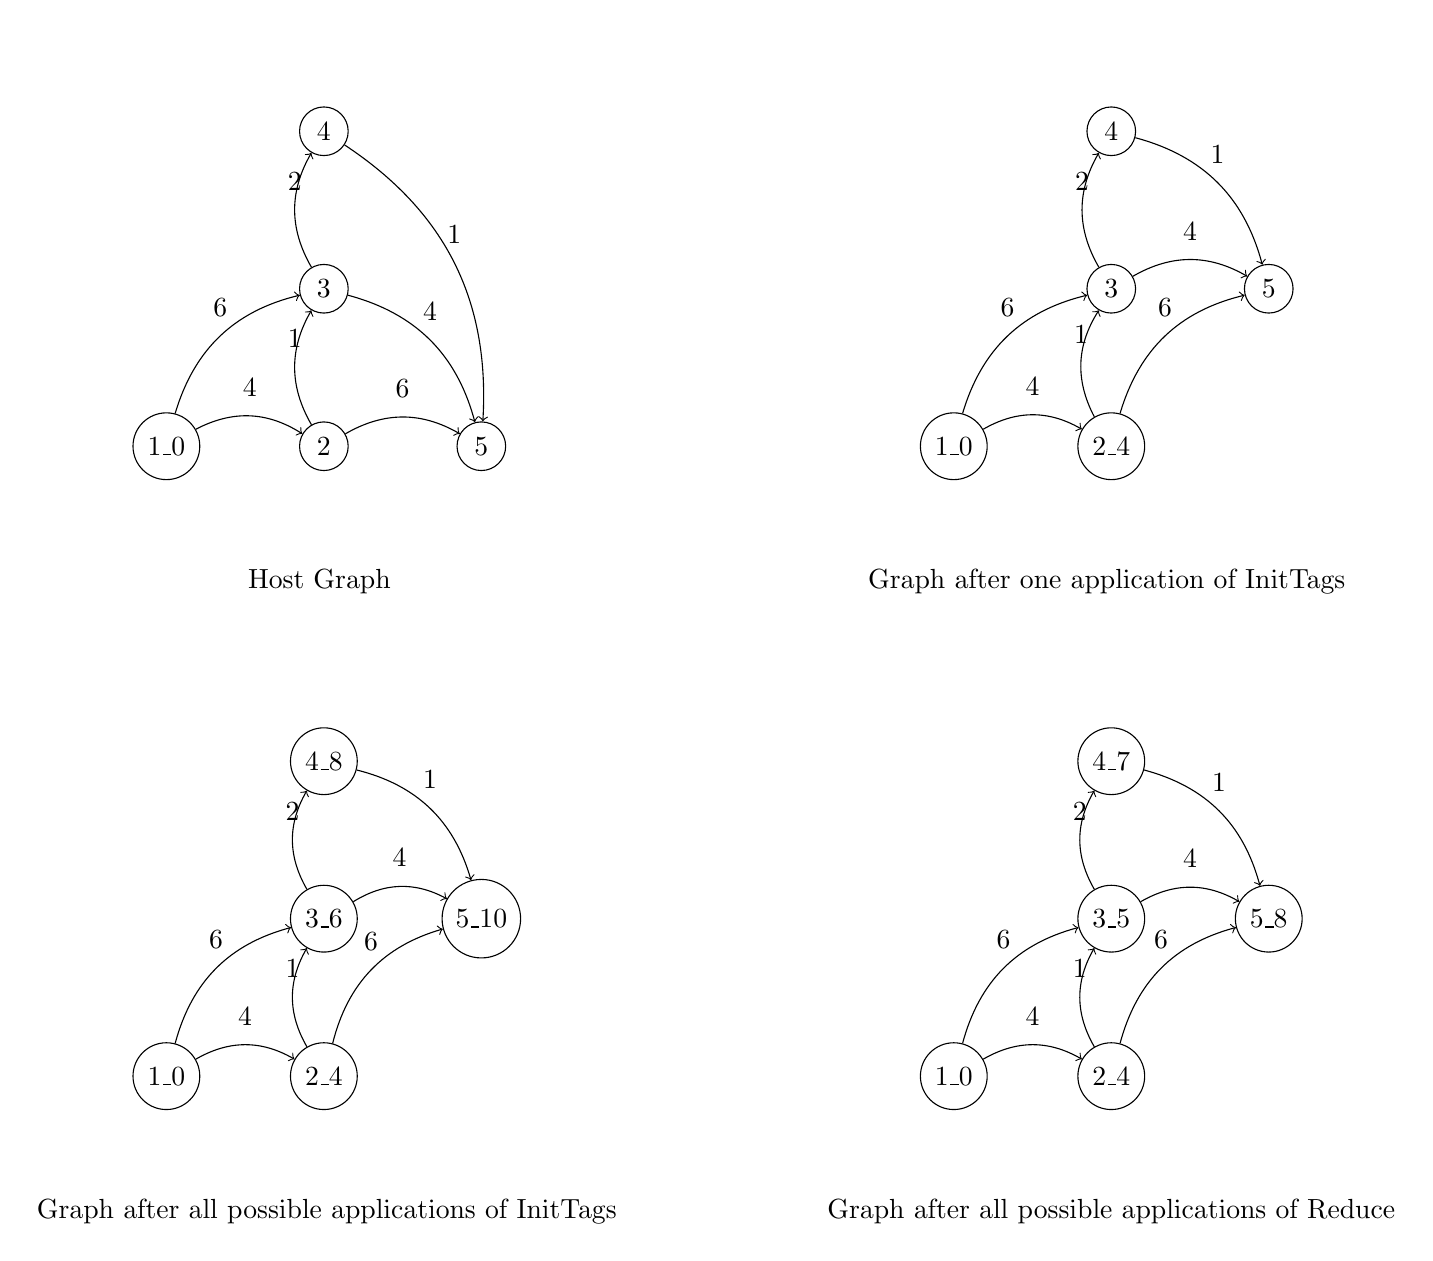
\begin{tikzpicture}[scale=2]
  \node (n1_1) [vertex] at (0, 4) {$1\_0$};
  \node (n1_2) [vertex] at (1, 4) {2};
  \node (n1_3) [vertex] at (1, 5) {3};
  \node (n1_4) [vertex] at (1, 6) {4};
  \node (n1_5) [vertex] at (2, 4) {5};
  \path [edge] (n1_1) edge node[label=above:{4}] {} (n1_2);
  \path [edge] (n1_1) edge node[label=above:{6}] {} (n1_3);
  \path [edge] (n1_2) edge node[label=above:{1}] {} (n1_3);
  \path [edge] (n1_3) edge node[label=above:{2}] {} (n1_4);
  \path [edge] (n1_2) edge node[label=above:{6}] {} (n1_5);
  \path [edge] (n1_3) edge node[label=above:{4}] {} (n1_5);
  \path [edge] (n1_4) edge node[label=above:{1}] {} (n1_5);
  \node (g0) [rule, fit={(n1_1) (n1_2) (n1_3) (n1_4) (n1_5)}, label=below:{Host Graph}] {};
  
  \node (n2_1) [vertex] at (5, 4) {$1\_0$}; % probably have to change these coordinates.
  \node (n2_2) [vertex] at (6, 4) {$2\_4$};
  \node (n2_3) [vertex] at (6, 5) {3};
  \node (n2_4) [vertex] at (6, 6) {4};
  \node (n2_5) [vertex] at (7, 5) {5};
  \path [edge] (n2_1) edge node[label=above:{4}] {} (n2_2);
  \path [edge] (n2_1) edge node[label=above:{6}] {} (n2_3);
  \path [edge] (n2_2) edge node[label=above:{1}] {} (n2_3);
  \path [edge] (n2_3) edge node[label=above:{2}] {} (n2_4);
  \path [edge] (n2_2) edge node[label=above:{6}] {} (n2_5);
  \path [edge] (n2_3) edge node[label=above:{4}] {} (n2_5);
  \path [edge] (n2_4) edge node[label=above:{1}] {} (n2_5);
  \node (g1) [rule, fit={(n2_1) (n2_2) (n2_3) (n2_4) (n2_5)}, label=below:{Graph after one application of InitTags}] {};
  
  \node (n3_1) [vertex] at (0, 0) {$1\_0$}; % probably have to change these coordinates.
  \node (n3_2) [vertex] at (1, 0) {$2\_4$};
  \node (n3_3) [vertex] at (1, 1) {$3\_6$};
  \node (n3_4) [vertex] at (1, 2) {$4\_8$};
  \node (n3_5) [vertex] at (2, 1) {$5\_10$};
  \path [edge] (n3_1) edge node[label=above:{4}] {} (n3_2);
  \path [edge] (n3_1) edge node[label=above:{6}] {} (n3_3);
  \path [edge] (n3_2) edge node[label=above:{1}] {} (n3_3);
  \path [edge] (n3_3) edge node[label=above:{2}] {} (n3_4);
  \path [edge] (n3_2) edge node[label=above:{6}] {} (n3_5);
  \path [edge] (n3_3) edge node[label=above:{4}] {} (n3_5);
  \path [edge] (n3_4) edge node[label=above:{1}] {} (n3_5);
  \node (gx) [rule, fit={(n3_1) (n3_2) (n3_3) (n3_4) (n3_5)}, label=below:{Graph after all possible applications of InitTags}] {}; 
  
  \node (n4_1) [vertex] at (5, 0) {$1\_0$}; % probably have to change these coordinates.
  \node (n4_2) [vertex] at (6, 0) {$2\_4$};
  \node (n4_3) [vertex] at (6, 1) {$3\_5$};
  \node (n4_4) [vertex] at (6, 2) {$4\_7$};
  \node (n4_5) [vertex] at (7, 1) {$5\_8$};
  \path [edge] (n4_1) edge node[label=above:{4}] {} (n4_2);
  \path [edge] (n4_1) edge node[label=above:{6}] {} (n4_3);
  \path [edge] (n4_2) edge node[label=above:{1}] {} (n4_3);
  \path [edge] (n4_3) edge node[label=above:{2}] {} (n4_4);
  \path [edge] (n4_2) edge node[label=above:{6}] {} (n4_5);
  \path [edge] (n4_3) edge node[label=above:{4}] {} (n4_5);
  \path [edge] (n4_4) edge node[label=above:{1}] {} (n4_5);
  \node (gn) [rule, fit={(n4_1) (n4_2) (n4_3) (n4_4) (n4_5)}, label=below:{Graph after all possible applications of Reduce}] {}; 
  
\end{tikzpicture}
\caption{Simple Dijkstra Program Example}
\end{figure}

\restoregeometry

\section{GP2 Compiler}
GP2 has a number of differences in the way in which it was implemented. As well as trying to address the issues of maintainability and usability, several features were added. %TODO ~AMMEND: differences to what? We're not comparing to GP1. Say what it does and why it was made.
Instead of using an abstract machine, the GP2 compiler generates C code directly \cite{chris_compiler}, which removes the reliance on YAM, the YAM compiler, and YAM graph and program formats. It means that any C compiler can be used to generate the bytecode. It also attempts to standardise and document the format of graphs and programs that it takes. This means that tools to generate graphs either graphically or programmatically can be created without reducing modularity or creating complexity and interdependance between the components of the system \cite{gp2_ide}.

GP2 no longer enforces non-detereministic execution \cite[p. 15]{gp2_ide}, and doesn't backtrack to reach all possible solutions. This was done to achieve a higher level of implementation efficiency \cite[p. 15]{chris_compiler}, but sacrifices completeness.

The GP2 compiler parses the program and host graph files, and generates a C code representation of the program, which can then be run. % It generates an AST for the program, and creates files for each rule, with methods for matching, and methods for applying.

%TODO ~ADD: more detailed explanation of how the GP2 compiler works.

\section{GP2 Editor}
%TODO ~ADD: a screenshot
The GP2 graphical editor for creating graphs and graph programs is currently under development. It will allow for the creation of graphs graphically, rather than textually, and it will allow for the creation of programs textually, and their rules graphically, assigning the LHS and RHS of the rules. In contrast with the GP1 editor, the GP2 editor will also include functionality to highlight nodes. %TODO ~MENTION: marks, rather than highlighting nodes.

\section{Program Tracing}
There are several techniques available to software developers when attempting to track down the locations of errors they've made. This process is called debugging, and many of the techniques involve outputting information about the program and its state throughout its execution. Other techniques involve dumping the last-stable memory at the point of a program crashing, which will then be analysed. 

\subsection{Tracing}
Tracing through the steps of a program has been around since programs themselves. The BASIC programming language had a command \emph{TRON}, short for TRace ON, which print the line numbers of each command as the program ran. 
Tracing allows programmers to ensure that each step is procuding the right results and allows a more detailed insight into the workings of a program. This is done by logging information about the execution of a program that will be useful for debugging or diagnostics, formal methods of which have been discussed as far back as the 70s \cite{psych_debug, code_walkthroughs}.

Although tracing, when as simple as possible, can be merely the addition of a few print statements, when applied throughout a program as a debugging tool, because tracing is generally such a low-level process, there's potential for a vast amount of logging messages \cite{}, which can impact performance. Usually programs have either run-time or compile-time options for turning off debugging to combat this. %TODO ~FIND: a paper or reference for the empty citation.

The trace is also usually only seen by the developer of a system, and so there is no need to have the messages be readable by, or understandable to, the users. This means it can be cheap to implement. However, due to the fact that tracing is a cross-cutting concern \cite{}, meaning that is is involved all throughout the program, it's had to decouple and modularise. %TODO ~FIND: a paper or reference for the empty citation.

The points within the program where information is divulged are referred to as tracepoints. They are hooking mechanisms which allow for tracing with little overhead when disabled, but that can be enabled at run-time and will provide static tracing \cite{tracing_book}.

\subsection{Breakpoints}
Breakpoints allow for the stopping or pausing of a program part of the way through its execution. This is done to allow usually to obtain knowledge about the state of the program at certain points throughout the process. \emph{Instruction Breakpoints} interrupt the program before an instruction is executed, but there are also \emph{Conditional Breakpoints}, or \emph{Watchpoints}, which trigger upon events such as reading from, or writing to, specific memory locations, or upon certain keystrokes.

%TODO ~FIND: some papers on debugging
%TODO ~READ: psych_debug and code_walkthroughs for stuff to say about tracing/debugging
%TODO ~READ: https://bitbucket.org/pypy/extradoc/src/tip/talk/pepm2011/bolz-allocation-removal.pdf (reference #16 might be good)

%TODO ~FIND, ~MENTION: a paper on TRON and mention it briefly.

% END OF LITERATURE REVIEW

\chapter{Design}
\section{Users \& Requirements}
% ~2000 words (Problem analysis)
% ~3333 words (between Design *and* Implementation)

The users of GP2 as it stands are predominantly students and staff at the University of York, and researchers in the field of graph transformations. The students use it to get a hands-on appreciation of both graph transformation generally, and GP2 specifically.

%TODO ~ADD: What users care about. Students want usablility. Also no performance impact. Developers want maintainability and integratability.

Any tracing will need to not have any negative impacts on the currently existing system. Ideally, as little effect on efficiency and performace as possible should be made to the compiler, and to the generated code running the Graph Program. The new system should also be completely backwards compatible. That is, the tracing should be optional, with the current implementation for running a given graph program on a host graph still performing that action.

Also, any changes made to the editor should serve only to enhance the user's understanding of the underlying process, and should be avoidable if they so choose.

It is critical to correctly identify the requirements for a system to be determined succesful to allow for any evaluation. It also means that throughout the design process, there are key features to be kept in mind.
\begin{enumerate}
	\item A program must be able to be stepped through, that is, a portion of the program (step) must be able to be run on either the host graph, or the resultant graph of a previous step's execution.
	\item These steps would ideally be of specifiable sizes.
	\item These steps must be able to be displayed graphically in the GP2 Editor.
	\item These steps would ideally be displayed in such a way to highlight themselves.
\end{enumerate}

\section{High-Level Design}
Writing maintainable code involves ensuring that the intent behind each procedure is as clear as possible to a programmer, familiar or unfamiliar with the system. This can be done with clear and useful naming of variables and functions, and with appropriate levels of comments documenting the intent behind the code.

% I try to not have an impact on the existing code. No impact on performance. No impact on flow or structure.

%TODO ~ADD: ideas i was gonna do, but didn't. alternative implementations
% I was gonna have the compiler create a chunk of runnable code. But that means having the compiler run for each step. 
% Or maybe the compiler could create chunks of runnable code, sub-programs. But this would slow down the execution as there would be more file I/O calls. And causes more distruption to the running of a program if the entire program is being run.

% So let's be sensible and implement breakpoints after every command, and sort the breakpoints into sizes, which correspond to step sizes.

% I use labels to identify which nodes and edges have been added, or matched.
%TODO ~CHECK: That this is a valid use of labels. Check that there's no "has_empty_label" check that would be broken by my "highlighting".

\section{Design in more detail} %TODO ~AMMEND: This title to something a bit catchier and more informative.

% Have to know when to stop.
% Have to use the previously outputted graph. But only if we've stepped through.
% Have to know when to start, if we've previously only stepped through a bit.
% Add a very small file that holds the number of where to start. Its existence mean to use the previously outputted graph.
% Adds a small brief File I/O cost at the beginning, but that's when the graph is loaded anyway, and it's really minor. Like 3 lines? (one for current step, one for highlighted nodes, one for highlighted edges)
% Factor out the finalisation, as it can happen at other parts of the code now.
% Have matching without executing.

% Have to highlight changes somehow.
	% Could use a custom mark. But that means that it can't have a mark, or I'd have to change the language to allow for multiple marks.
	% Could use a file with highlighted nodes/edges, but that seems to disrupt the existing pipeline. Editor would need to load an additional file, jsut for the highlights.
	% Could have special designated labels for changes, but that may or may not change the behaviours of rules. And a record would still need to be made to remove them again.
	
% Choose the 2nd one. I/O still only needs to be done once at the beginning and once at the end, and only if steps are happening.
 
\chapter{Implementation}
% ~3333 words (between Design *and* Implementation)

% 1. Find the parts of the code that generate different sizes of step.
% 2. Implement breakpoints after each of them.

\begin{lstlisting}[label=code:breakpoint_1, caption=Pseudocode of breakpoints]
rule_step_application
if we_should_stop
	finalise
	exit
endif
\end{lstlisting}




\chapter{Evaluation}
% ~3333 words

% Relate back to requirements
% Talk about what I got done.
	% Stepping through
	% Various size steps
	% 
% Talk about what I didn't get done.

\section{Performance}
%TODO ~ADD: Performance Benchmarks


\chapter{Conclusion}
% ~1333 words
\section{Future Work}

% Have the Graphical Editor recognise the special labels and draw attention to changes.
% Stepping backwards?

\bibliography{references}

\chapter{Appendices}
\end{document}